\Needspace{12\baselineskip}
\section{Варианты YETI}
\label{app:variants}

\subsection{Почему требуется ограничивать локальную кривизну}

Само по себе условие $\norm{y-x^\ast}\le R$ не даёт полиномиальной
по $L_1R$ оценки отношения локальных констант гладкости.
Рассмотрим одномерную функцию
\[
 \varphi(t)=\cosh(L_1t).
\]
Она выпукла, имеет минимум в нуле и удовлетворяет
\[
 \varphi''(t)=L_1^2\cosh(L_1t)
 \le L_1^2+L_1|\varphi'(t)|.
\]
Однако
\[
 \frac{\varphi''(R)}{\varphi''(0)}=\cosh(L_1R)
\]
растёт экспоненциально. Поэтому одной принадлежности центров шару
недостаточно, чтобы убрать проверку кривизны и сохранить прежнюю
оценку числа обращений к оракулу при локальном вызове. Этот пример касается только используемого
решателя и не исключает существования других алгоритмов.

\subsection{Выбор стохастического градиента}

Пусть функции $\varphi_i$ имеют локальные константы гладкости $L_i>0$
на увеличенном шаре, а точки $x,w$ лежат в исходном шаре.
Для случайного индекса $I$ с вероятностями $q_i>0$
лемма~\ref{lem:local-bregman} даёт
\begin{equation}\label{eq:importance-variance}
 \begin{aligned}
 \mathbb E\left\|
 \frac{\nabla\varphi_I(x)-\nabla\varphi_I(w)}{nq_I}
 \right\|^2&=\frac1{n^2}\sum_i
       \frac{\norm{\nabla\varphi_i(x)-\nabla\varphi_i(w)}^2}{q_i}
 \\&\le\frac2{n^2}\sum_i\frac{L_i}{q_i}
       \bigl(\varphi_i(x)-\varphi_i(w)
                  -\ip{\nabla\varphi_i(w)}{x-w}\bigr).
 \end{aligned}
\end{equation}
Если
\[
 q_i=\frac{L_i}{\sum_jL_j},
\]
то последняя строка равна
\[
 \left(\frac2n\sum_iL_i\right)\frac1n\sum_i
 \bigl(\varphi_i(x)-\varphi_i(w)-\ip{\nabla\varphi_i(w)}{x-w}\bigr).
\]
При равномерной выборке стандартная верхняя оценка содержит
$2\max_iL_i$ вместо $2n^{-1}\sum_iL_i$.

Отношение этих величин может иметь порядок $n$ даже в рассматриваемом классе.
В одномерном случае при $L_0>0$ возьмём
\[
 \begin{gathered}
 f_1(t)=\frac{L_0}{2}(t-R)^2,\\
 f_i(t)=0\quad(i>1).
 \end{gathered}
\]
Зададим известные верхние оценки $L_{0,i}=L_0$ для всех $i$.
Выберем параметры
\[
 \begin{gathered}
 y=0,\\
 L_1R=n,\\
 r=\frac1{2L_1},\\
 \lambda=L_0.
 \end{gathered}
\]
Тогда константы из~\eqref{eq:local-smoothness}, то есть
\[
 L_i=e^{3L_1r}\bigl(L_{0,i}+L_1\norm{\nabla f_i(y)}\bigr)+\lambda,
\]
удовлетворяют
\[
 \frac{\max_iL_i}{n^{-1}\sum_iL_i}
 =\frac{1+e^{3/2}(1+n)}{1+2e^{3/2}}.
\]
Это отношение растёт линейно по $n$. Тем самым для данной оценки
внутреннего решателя неравномерная выборка существенна. Отсюда не следует,
что любой метод с равномерной выборкой обязательно проигрывает.

В решателе YETI используются вероятности
\[
 q_i=\frac{L_i}{\sum_jL_j}.
\]
Если другое распределение обеспечивает лишь
\[
 \frac{L_i}{nq_i}\le\frac cn\sum_jL_j,
\]
то в правой части оценки~\eqref{eq:importance-variance}
появляется множитель $c$. Его влияние на оценку сложности
следует учитывать вместе с выбором параметров эпохи.

Сохранение опорного градиента также существенно. При $a>0$ для функций
\[
 \begin{gathered}
 f_1(t)=\frac{(t-a)^2}{2},\\
 f_2(t)=\frac{(t+a)^2}{2}
 \end{gathered}
\]
минимум их среднего достигается в нуле, но
\[
 \frac12\sum_{i=1}^2|f_i'(0)|^2=a^2>0.
\]
Поэтому градиент случайно выбранной компоненты имеет в решении ненулевую
дисперсию. В оценке же~\eqref{eq:importance-variance}
разности градиентов обращаются в ноль при $x=w$.
Без поправки с помощью сохранённых градиентов дисперсия в решении
может оставаться положительной, и приведённое доказательство
геометрической сходимости неприменимо.

\subsection{Покомпонентные секущие для обобщённых линейных моделей}

Пусть
\[
 f_i(x)=\phi_i(a_i^{\mathsf T}x),
\]
где $\phi_i$ выпукла и дважды непрерывно дифференцируема.
По уже вычисленным градиентам в точках $x_0,x_1$ определим
\[
 \begin{gathered}
 s=x_1-x_0,\\
 \Delta g_i=\nabla f_i(x_1)-\nabla f_i(x_0).
 \end{gathered}
\]

\begin{proposition}[восстановление среднего гессиана]\label{prop:glm-secant}
Если $\ip{\Delta g_i}s>0$, то
\begin{equation}\label{eq:glm-secant}
 \frac{\Delta g_i\Delta g_i^{\mathsf T}}{\ip{\Delta g_i}s}
 =\int_0^1\nabla^2f_i(x_0+ts)\,dt.
\end{equation}
Если $a_i^{\mathsf T}s=0$, то нулевая секущая может соответствовать
ненулевой матрице в правой части. Если же средняя скалярная кривизна
равна нулю, а секущая явно определена как нулевая матрица (без деления
на ноль), то обе части равенства равны нулю.
\end{proposition}

\begin{proof}
По формуле Ньютона--Лейбница
\[
 \begin{aligned}
 \Delta g_i&=(a_i^{\mathsf T}s)a_i
     \int_0^1\phi_i''(a_i^{\mathsf T}(x_0+ts))\,dt,\\
 \ip{\Delta g_i}s&=(a_i^{\mathsf T}s)^2
     \int_0^1\phi_i''(a_i^{\mathsf T}(x_0+ts))\,dt,\\
 \int_0^1\nabla^2f_i(x_0+ts)\,dt
 &=a_i a_i^{\mathsf T}\int_0^1\phi_i''(a_i^{\mathsf T}(x_0+ts))\,dt.
 \end{aligned}
\]
При положительном знаменателе сокращение скалярных множителей
даёт~\eqref{eq:glm-secant}. При $a_i^{\mathsf T}s=0$
равенство $\Delta g_i=0$ не определяет интеграл от $\phi_i''$.
Если же этот интеграл равен нулю, то средний гессиан и разность градиентов нулевые.
\end{proof}

Таким образом, положительная компонентная секущая восстанавливает
средний гессиан вдоль отрезка. Чтобы получить гессиан в конце отрезка,
нужно дополнительное предположение.

\begin{proposition}[приближение гессиана пуассоновской модели]\label{prop:poisson-secants}
Пусть
\[
 f_i(x)=e^{a_i^{\mathsf T}x}-y_i a_i^{\mathsf T}x,
\]
где $y_i\ge0$ и $\norm{a_i}\le L_1$.
Эти компоненты удовлетворяют условию класса при
\[
 L_{0,i}=y_i\norm{a_i}^2.
\]
Если для каждого ненулевого $a_i$ выполнено $a_i^{\mathsf T}s\ne0$,
то матрица $M$, полученная усреднением секущих~\eqref{eq:glm-secant},
удовлетворяет
\begin{equation}\label{eq:poisson-secant-comparison}
 e^{-L_1\norm s}\nabla^2f(x_1)
 \preceq M\preceq e^{L_1\norm s}\nabla^2f(x_1).
\end{equation}
Нулевым $a_i$ в сумме соответствуют нулевые матрицы.
\end{proposition}

\begin{proof}
Непосредственно из вида компоненты получаем
\[
 \norm{\nabla^2f_i(x)}
 =e^{a_i^{\mathsf T}x}\norm{a_i}^2
 \le y_i\norm{a_i}^2+|e^{a_i^{\mathsf T}x}-y_i|\norm{a_i}^2
 \le L_{0,i}+L_1\norm{\nabla f_i(x)}.
\]
Кроме того, для $0\le t\le1$ по неравенству Коши--Буняковского--Шварца
\[
 |a_i^{\mathsf T}(x_0+ts-x_1)|\le L_1\norm s.
\]
Поэтому
\[
 e^{-L_1\norm s}e^{a_i^{\mathsf T}x_1}
 \le e^{a_i^{\mathsf T}(x_0+ts)}
 \le e^{L_1\norm s}e^{a_i^{\mathsf T}x_1}.
\]
Умножив на положительно полуопределённую матрицу
$a_i a_i^{\mathsf T}$, проинтегрировав и усреднив по $i$,
получаем~\eqref{eq:poisson-secant-comparison}.
\end{proof}

Для применения основной теоремы нужны также
предположения~\ref{asm:minimizer}--\ref{asm:heterogeneity}.
Условие отсутствия пропущенных ненулевых направлений существенно:
если $a_i^{\mathsf T}s=0$ при $a_i\ne0$, то градиентная секущая нулевая,
а гессиан пуассоновской компоненты ненулевой.
Кроме того, две наблюдаемые параллельные производные не доказывают, что
компонента глобально представима в виде $\phi_i(a_i^{\mathsf T}x)$.
Поэтому восстановленную матрицу можно использовать для выбора
эвристического предложения YETI: проверки и основные итерации метода
сохраняют оценку его сложности.
Замена полной суммы секущих выборкой фиксированного числа компонент
потребовала бы отдельной теоремы о спектральном приближении.

\subsection{Ограничение числа запросов эвристики к оракулу}
\label{sec:budget}

Пусть $B_0=n\lceil\log N\rceil$, $G$ --- суммарное число запросов к оракулу
в основных итерациях, $H$ --- в эвристических блоках.
Выберем $\omega\ge0$. Перед очередным эвристическим блоком разрешим
\begin{equation}\label{eq:adaptive-cheap-budget}
 B_k=n\left\lfloor
       \frac{\min\{B_0,B_0+\omega G-H\}}n
       \right\rfloor
\end{equation}
запросов. Если $B_k<n$, блок пропускается. Перед каждым вычислением функции и полного градиента
оставляют $n$ запросов. Все обращения эвристики к оракулу, включая
проверки предложенных точек, учитываются в счётчике $H$.

Доказательство следующей теоремы сводится к пошаговой проверке инварианта
и приведено в приложении~\ref{app:budget-proof}.

\proofdown{thm:adaptive-cheap-budget}
\begin{theorem}[число запросов эвристики]
\label{thm:adaptive-cheap-budget}
Если к некоторому моменту работы начато $k$ эвристических
блоков, то в этот момент выполнено
\begin{equation}\label{eq:budget-prefix-invariant}
 H\le\min\{kB_0,B_0+\omega G\}.
\end{equation}
Правило~\eqref{eq:adaptive-cheap-budget} сохраняет верхнюю оценку
теоремы~\ref{thm:cheap-upper}. Кроме того,
\begin{equation}\label{eq:adaptive-budget-total}
 \mathbb E T\le B_0+(1+\omega)\mathbb E G.
\end{equation}
Здесь все заключительные вычисления функции и полного градиента включены в $G$ или $H$.
\end{theorem}

При $\omega=1$ эвристика сверх первых $B_0$ запросов не может сделать
больше обращений к оракулу, чем уже сделали основные итерации. Первому блоку доступны все $B_0$ запросов,
поэтому при одинаковых значениях случайных величин он выполняет
те же запросы, что и блок с постоянным ограничением $B_0$.
Это не требует предположения о полезности эвристики.
Ограничение числа запросов существенно: повторение одной и той же точки без
остановки и без перехода к основной итерации может сделать
число обращений к оракулу бесконечным, даже если значение функции не возрастает.


\clearpage
\section{Подробное описание YETI}\label{app:implementation}
\subsection{Критерий остановки по истории запросов}

Вычисление функции и полного градиента в точке $p\in\mathbb R^d$ даёт аффинную миноранту
$u\mapsto f(p)+\ip{\nabla f(p)}{u-p}$. Её минимум по $u\in B(0,R)$
равен
\begin{equation}\label{eq:history-full-lower}
 \widetilde f(p)
 =f(p)-\ip{\nabla f(p)}p-R\norm{\nabla f(p)}.
\end{equation}
Это нижняя оценка оптимального значения:
\[
 f^\ast\by{\ge}{\text{\ref{asm:components}}} f(p)+\ip{\nabla f(p)}{x^\ast-p}
 \by{\ge}{\text{\ref{asm:minimizer}}}
 f(p)-\ip{\nabla f(p)}p-R\norm{\nabla f(p)}.
\]
Во втором переходе использовано также неравенство Коши--Буняковского--Шварца.
Если $p\in B(0,R)$, то разность $f(p)-\widetilde f(p)$ является
зазором Франка--Вульфа~\citep{jaggi2013}; оценка $\widetilde f(p)\le f^\ast$
верна и при $p\notin B(0,R)$.
Обозначим через $\widetilde f_{\rm best}$ максимум всех сохранённых
нижних оценок, а через $w_{\rm best}$ --- лучшую из точек шара $B(0,R)$,
в которых известно значение функции. Метод останавливается и возвращает
$w_{\rm best}$, если
\begin{equation}\label{eq:history-stop}
 f(w_{\rm best})-\widetilde f_{\rm best}\le\varepsilon/2.
\end{equation}
Точка $w_{\rm best}$ хранится отдельно от $x$: при ускоренном обновлении $x$
значение функции не обязательно убывает монотонно.
Все вычисления функции и полного градиента выполняются подпрограммой \textsc{Оценка}
(алгоритм~\ref{alg:pass}): в предложенных эвристикой точках,
в центрах, в опорных и проверочных точках решателя. Если значения и градиенты всех компонент в данной точке уже
известны, повторные запросы не нужны. Для проверки~\eqref{eq:history-stop}
достаточно хранить $\widetilde f_{\rm best}$, $w_{\rm best}$
и $f(w_{\rm best})$; эвристика может хранить и дополнительные данные для выбора точек.

\begin{algorithm}[H]
\caption{\textsc{Оценка}$(p)$: вычисление функции, градиента и проверка точности}\label{alg:pass}
\begin{algorithmic}[1]
\Require точка $p$
\State запросить $\bigl(f_i(p),\nabla f_i(p)\bigr)$ для всех $i$, для которых ответы в точке $p$ ещё не получены
\State $\widetilde f_{\rm best}\gets\max\bigl\{\widetilde f_{\rm best},\ f(p)-\ip{\nabla f(p)}p-R\norm{\nabla f(p)}\bigr\}$
\If{$\norm p\le R$ и $f(p)<f(w_{\rm best})$} \Comment{до первой такой точки $f(w_{\rm best})=+\infty$}
 \State $w_{\rm best}\gets p$
\EndIf
\If{$f(w_{\rm best})-\widetilde f_{\rm best}\le\varepsilon/2$}
 \State завершить YETI с ответом $w_{\rm best}$
\EndIf
\end{algorithmic}
\end{algorithm}

\proofdown{lem:history-small-gradient}
\begin{lemma}[остановка при малом субградиенте]
\label{lem:history-small-gradient}
Пусть $z\in B(0,R)$, функция и полный градиент в $z$ уже вычислены и
$g=\nabla f(z)+v_z$, где $v_z\in N_{B(0,R)}(z)$. Тогда
\[
 f(z)-\widetilde f(z)\le2R\norm g.
\]
В частности, при $\norm g\le\varepsilon/(4R)$ после записи $z$
в историю выполнено~\eqref{eq:history-stop}.
\end{lemma}

Для проверки остановки можно использовать и ответы компонент,
полученные в разных точках. Соответствующая нижняя оценка и способ её
пересчёта без новых запросов приведены в
приложении~\ref{app:component-history}. Эта возможность используется
эвристикой в экспериментах, но для оценки сложности YETI не нужна.

\subsection{Оценка локальной кривизны}

После вычисления функции и полного градиента в $y$ известна величина
\begin{equation}\label{eq:observed-curvature}
 \ell(y)=\frac1n\sum_{i=1}^n
       \bigl(L_{0,i}+L_1\norm{\nabla f_i(y)}\bigr).
\end{equation}
\proofdown{lem:observed-curvature}
\begin{lemma}[оценка кривизны через невязку]\label{lem:observed-curvature}
При предположениях~\ref{asm:components}--\ref{asm:minimizer}
и~\ref{asm:heterogeneity} для любой точки $y$
\begin{equation}\label{eq:curvature-gap}
 \begin{gathered}
 \norm{\nabla f(y)}
 \le L_1\bigl(\delta+f(y)-f^\ast\bigr)
 +\sqrt{2L_0\bigl(\delta+f(y)-f^\ast\bigr)},\\
 L_1\norm{\nabla f(y)}\le\ell(y),\\
 \ell(y)\le\tfrac32L_0+2L_1^2\bigl(\delta+f(y)-f^\ast\bigr).
 \end{gathered}
\end{equation}
Кроме того, для любых $x,y$
\begin{equation}\label{eq:curvature-transfer}
 \begin{gathered}
 \ell(x)\le e^{L_1\norm{x-y}}\ell(y),\\
 \norm{\nabla^2f(x)}\le\ell(x).
 \end{gathered}
\end{equation}
В частности, для любого $r>0$ на $B(y,3r)$ норма гессиана компоненты $f_i$
не превосходит
\begin{equation}\label{eq:component-local-smoothness}
 e^{3L_1r}\bigl(L_{0,i}+L_1\norm{\nabla f_i(y)}\bigr).
\end{equation}
\end{lemma}

\begin{corollary}[нижняя оценка невязки по кривизне]\label{cor:curvature-lower-gap}
Вычисление функции и полного градиента в $y$ даёт нижнюю оценку невязки по функции
\[
 f(y)-f^\ast\ge
 \frac{\ell(y)-\tfrac32L_0-2L_1^2\delta}{2L_1^2}.
\]
Если правая часть отрицательна, оценка тривиальна.
\end{corollary}


\subsection{Параметры YETI}
Состояние метода состоит из точек $x,v\in B(0,R)$, числа
$\mathcal A>0$ и параметра $h>0$. Число $\mathcal A$ играет ту же роль,
что и сумма коэффициентов $A_k$ в ускоренных методах с оценочными
последовательностями: ниже доказано, что всегда
$f(x)-f^\ast\le R^2/\mathcal A$, а число $\mathcal A$ не убывает
и увеличивается при обновлении~\eqref{eq:damped-update}.
В отличие от введённой в обозначениях суммы $A_k$, начальное значение
$\mathcal A$ положительно. Радиус $r$ выбирается так, чтобы на малом шаре кривизна менялась
не более чем в постоянное число раз. Проксимальный параметр
ограничивается снизу по трём причинам, связанным с коэффициентом
ускоренного шага, обусловленностью локальной задачи и остановкой.
Используем следующие значения:
\begin{equation}\label{eq:outer-parameters}
 \begin{aligned}
 &r=\min\left\{R,\frac1{2L_1}\right\},\\
 &\lambda_\downarrow(\mathcal A)
 =\max\left\{\frac{1-\frac12(r/R)^{2/3}}{\frac14(r/R)^{4/3}\mathcal A},\
       \frac1n\Bigl(\frac32L_0+2L_1^2\Bigl(\delta+\frac{R^2}{\mathcal A}\Bigr)\Bigr),\
       \frac\varepsilon{8rR}\right\},\\
 &\lambda_{\uparrow}=\lambda_\downarrow\Bigl(\frac{R^2}{2\Delta}\Bigr).
 \end{aligned}
\end{equation}
Здесь $r$ --- радиус малого шара, $\lambda_\downarrow(\mathcal A)$ ---
нижняя граница проксимального параметра, $\lambda_{\uparrow}$ --- верхняя.
Три выражения под знаком максимума отвечают этим причинам: первое не даёт
коэффициенту $\alpha$ ускоренного шага превысить $\frac12(r/R)^{2/3}$, второе делает
локальную задачу хорошо обусловленной, третье нужно для остановки.

Метод начинает работу с $x=v=0$, $\mathcal A=R^2/(2\Delta)$, $h=\lambda_{\uparrow}$ и пустой
историей запросов.

\subsection{Основная итерация YETI}
В состоянии $(x,v,\mathcal A,h)$ вычисляются
\begin{equation}\label{eq:outer-step-setup}
 \begin{aligned}
 &\lambda=\min\bigl\{\max\{h,\lambda_\downarrow(\mathcal A)\},\lambda_{\uparrow}\bigr\},\\
 &a_\lambda=\frac{1+\sqrt{1+4\lambda\mathcal A}}{2\lambda},\\
 &\alpha=\frac{a_\lambda}{\mathcal A+a_\lambda},\\
 &y=(1-\alpha)x+\alpha v.
 \end{aligned}
\end{equation}
Число $a_\lambda$ --- положительный корень уравнения
$\lambda a_\lambda^2=\mathcal A+a_\lambda$, поэтому
\[
 \begin{gathered}
 \lambda\mathcal A\alpha^2=1-\alpha,\\
 \lambda a_\lambda=1/\alpha.
 \end{gathered}
\]
По значениям градиентов компонент в $y$ проверяется условие на кривизну:
\begin{equation}\label{eq:simple-curvature-test}
 \ell(y)\le e^{L_1r}\Bigl(\frac32L_0+2L_1^2\Bigl(\delta+\frac{R^2}{\mathcal A}\Bigr)\Bigr).
\end{equation}
Если это условие нарушено, то по следствию~\ref{cor:curvature-lower-gap}
невязка в $y$ велика, и полупространство
\begin{equation}\label{eq:cut-update}
 \mathcal H_y=\left\{w:\ \ip{\nabla f(y)}{w-y}
 \le-\frac{\ell(y)-\frac32L_0-2L_1^2\delta}{2L_1^2}\right\}
\end{equation}
содержит точку минимума. В этом случае выполняется обновление
\[
 \begin{aligned}
 v^+&=\Pi_{B(0,R)}\Pi_{\mathcal H_y}v,\\
 h^+&=2\lambda,
 \end{aligned}
\]
при котором $x$ и $\mathcal A$ не меняются. Такой шаг называется
повышающим.

Если условие~\eqref{eq:simple-curvature-test} выполнено, запускается
локальный решатель (алгоритм~\ref{alg:local-solver}), использующий уже
полученные значения и градиенты компонент в $y$. Он возвращает точку $z$, субградиент $g$
задачи на шаре $B(0,R)$ в точке $z$ и число $\beta\ge0$.
Если $g$ мал, метод возвращает $z$. Иначе, положив $\gamma=\lambda/(\lambda+\beta)$,
уменьшаем вес ускоренного обновления, умножая его на $\gamma$,
по схеме из~\citep{carmon2022adaptive}:
\begin{equation}\label{eq:damped-update}
 \begin{aligned}
 \mathcal A^+&=\mathcal A+\gamma a_\lambda,\\
 x^+&=\frac{(1-\gamma)\mathcal A x+
                 \gamma(\mathcal A+a_\lambda)z}{\mathcal A^+},\\
 v^+&=\Pi_{B(0,R)}(v-\gamma a_\lambda g),\\
 h^+&=\begin{cases}2\lambda,&\beta>0,\\\lambda/2,&\beta=0.\end{cases}
 \end{aligned}
\end{equation}
Шаг при $\beta>0$ также называется повышающим, при $\beta=0$ ---
понижающим. При $\mathcal A^+\ge2R^2/\varepsilon$ метод возвращает $x^+$.

\subsection{Эвристический блок}\label{sec:heuristic-block}

Эвристика использует известные параметры задачи, историю ответов
оракула и собственные случайные величины. Каждый блок возвращает
управление за конечное число вычислений. Ограничение $n\lceil\log N\rceil$
распространяется на все запросы, включая запросы в отвергнутых точках и начальное
вычисление функции и полного градиента в $x$. Перед вызовом эвристики
резервируются $n$ запросов для проверки предложения.

Точка $z$ принимается, если $z\in B(0,R)$ и $f(z)\le f(x)$;
при этом меняется только $x$. Остановка возможна по критерию~\eqref{eq:history-stop}.
Решения, принимаемые эвристикой, измеримы. Для индексов локального решателя используются
новые независимые случайные величины; при заданной истории индексы имеют
распределение из раздела~\ref{sec:local-solver}.

\begin{algorithm}[H]
\caption{\textsc{Блок}$(x)$: эвристический блок}\label{alg:block}
\begin{algorithmic}[1]
\Require точка $x\in B(0,R)$, эвристика
\State $b=n\lceil\log N\rceil$ \Comment{каждый запрос уменьшает $b$ на единицу}
\State \Call{Оценка}{$x$}
\While{$b\ge n$ и эвристика не завершила блок}
 \State эвристика делает не более $b-n$ запросов и предлагает $z\in B(0,R)$
 \State \Call{Оценка}{$z$}
 \If{$f(z)\le f(x)$}
  \State $x\gets z$
 \EndIf
\EndWhile
\State \Return $x$
\end{algorithmic}
\end{algorithm}


\section{Локальное решение методом SVRG}\label{app:solver-implementation}
\subsection{Локальная задача}
Пусть $y\in B(0,R)$, $\lambda>0$ и $r>0$. Рассмотрим функции
\begin{equation}\label{eq:local-problem}
 \begin{aligned}
 P(z)&=f(z)+\frac\lambda2\norm{z-y}^2,\\
 P_i(z)&=f_i(z)+\frac\lambda2\norm{z-y}^2,
 \end{aligned}
\end{equation}
множество $\mathcal K=B(0,R)\cap B(y,r)$ и точку
\[
 u=\argmin_{z\in\mathcal K}P(z).
\]
Множество $\mathcal K$ компактно и выпукло, а $P$ сильно выпукла с параметром
$\lambda$, поэтому $u$ существует и единственна. Вычисление функции и полного градиента в $y$
позволяет найти числа
\begin{equation}\label{eq:local-smoothness}
 L_i=e^{3L_1r}\bigl(L_{0,i}+L_1\norm{\nabla f_i(y)}\bigr)+\lambda
\end{equation}
и их среднее
\[
 \overline L=\frac1n\sum_iL_i=e^{3L_1r}\ell(y)+\lambda.
\]
По лемме~\ref{lem:observed-curvature} норма гессиана $P_i$ на $B(y,3r)$
не превосходит $L_i$.

Следующая лемма описывает проекцию на $\mathcal K$ и локальную
кокоэрцитивность компонент; её доказательство приведено
в приложении~\ref{app:local-proofs}.

\proofdown{lem:local-projection}
\begin{lemma}[проекция на пересечение шаров]\label{lem:local-projection}
Если $z=\Pi_{\mathcal K}(b)$, то существуют такие $\xi,\zeta\ge0$, что
\begin{equation}\label{eq:two-ball-normal}
 \begin{gathered}
 b-z=\xi z+\zeta(z-y),\\
 \xi>0\Longrightarrow\norm z=R,\\
 \zeta>0\Longrightarrow\norm{z-y}=r.
 \end{gathered}
\end{equation}
Для $x,t\in B(y,r)$ выполнено
\begin{equation}\label{eq:local-bregman}
 \norm{\nabla P_i(x)-\nabla P_i(t)}^2
 \le2L_i\bigl(P_i(x)-P_i(t)-\ip{\nabla P_i(t)}{x-t}\bigr).
\end{equation}
В частности, градиент $P$ на $B(y,r)$ является $1/\overline L$-кокоэрцитивным.
\end{lemma}

\subsection{Эпоха SVRG}
В пределах одного вызова решателя величины $\lambda$, $y$ и $L_i$ не меняются. Индекс $i$ выбирается с вероятностью $L_i/(n\overline L)$.
Шаг и длина эпохи равны
\begin{equation}\label{eq:svrg-parameters}
 \begin{aligned}
 h_s&=\frac1{6\overline L},\\
 M&=\left\lceil\frac{21\overline L}{5\lambda}\right\rceil.
 \end{aligned}
\end{equation}
Так как $L_i\ge\lambda>0$, все вероятности $L_i/(n\overline L)$ положительны и их сумма равна единице.
В опорной точке $s\in\mathcal K$ известны значения и градиенты всех компонент. Из текущей точки
$x_j$ делается шаг с новым индексом $i_j$, условно независимым от предыдущих:
\begin{equation}\label{eq:svrg-step}
 \begin{aligned}
 &v_{i_j}=\nabla P(s)+\frac{\nabla P_{i_j}(x_j)-\nabla P_{i_j}(s)}{L_{i_j}/\overline L},\\
 &x_{j+1}=\Pi_{\mathcal K}(x_j-h_sv_{i_j}).
 \end{aligned}
\end{equation}
Следующая эпоха начинается в точке $w^+=x_M$, а новая опорная точка равна
\begin{equation}\label{eq:svrg-average}
 s^+=\frac{\sum_{j=0}^{M-1}(1-h_s\lambda)^{M-1-j}x_j}
          {\sum_{j=0}^{M-1}(1-h_s\lambda)^j}.
\end{equation}
Первая эпоха вызова начинается с $w=s=y$. Градиенты компонент
в опорной точке сохраняются, поэтому один внутренний шаг требует
одного запроса.


\begin{algorithm}[H]
\caption{\textsc{Эпоха}$(w,s)$: эпоха SVRG для локальной задачи}\label{alg:svrg-epoch}
\begin{algorithmic}[1]
\Require точки $w,s\in\mathcal K$, ответы всех компонент в точке $s$,
$P_i$, $\mathcal K$, $L_i$, $\overline L$, $h_s$, $M$ из алгоритма~\ref{alg:local-solver}
\State $x_0=w$
\For{$j=0,\dots,M-1$}
 \State выбрать индекс $i_j=i$ с вероятностью $L_i/(n\overline L)$ независимо от прошлого
 \State запросить $\nabla f_{i_j}(x_j)$
 \State $v_j=\nabla P(s)+\dfrac{\overline L}{L_{i_j}}\bigl(\nabla P_{i_j}(x_j)-\nabla P_{i_j}(s)\bigr)$
 \State $x_{j+1}=\Pi_{\mathcal K}(x_j-h_sv_j)$
\EndFor
\State \Return $\Bigl(x_M,\ \dfrac{\sum_{j=0}^{M-1}(1-h_s\lambda)^{M-1-j}x_j}{\sum_{j=0}^{M-1}(1-h_s\lambda)^j}\Bigr)$
\end{algorithmic}
\end{algorithm}

\subsection{Остановка локального решателя}
После эпохи вычисляется полный градиент в $w$. Сначала проверяется
набор
\[
 \begin{gathered}
 z=w,\\
 \beta=0,\\
 g=\nabla f(w),\\
 e=\nabla P(w).
 \end{gathered}
\]
Если он не принят, вычисляются точка и векторы
\begin{equation}\label{eq:certificate-projection}
 \begin{aligned}
 z&=\Pi_{\mathcal K}\bigl(w-\nabla P(w)/\overline L\bigr),\\
 e&=\nabla P(z)-\nabla P(w)+\overline L(w-z),\\
 g&=\nabla f(z)+\overline L\xi z,
 \end{aligned}
\end{equation}
и число
\[
 \beta=\overline L\zeta,
\]
где $\xi,\zeta$ --- коэффициенты из~\eqref{eq:two-ball-normal} именно для
проекции из первой строки. Для вычисления $e$ и $g$ нужен полный градиент
в $z$. В обоих случаях
\begin{equation}\label{eq:certificate-properties}
 \begin{gathered}
 g\in\partial(f+I_{B(0,R)})(z),\\
 e=g-(\lambda+\beta)(y-z),\\
 \beta>0\Longrightarrow\norm{y-z}=r,
 \end{gathered}
\end{equation}
где $I_{B(0,R)}$ --- индикаторная функция выпуклого множества; её
субдифференциал есть нормальный конус. Набор принимается, если
выполнено хотя бы одно из условий
\begin{equation}\label{eq:certificate-test}
 \begin{gathered}
 \norm g\le\frac\varepsilon{4R},\\
 \norm e\le\frac45(\lambda+\beta)\norm{y-z}.
 \end{gathered}
\end{equation}
Первое условие проверяется раньше второго.

Решатель целиком записан в алгоритме~\ref{alg:local-solver}.
Если после эпохи ни один набор не принят, то вычисляются функция и полный градиент
в новой опорной точке и начинается следующая эпоха.

\begin{algorithm}[H]
\caption{\textsc{Решатель}$(y,\lambda)$: приближённое решение локальной задачи}\label{alg:local-solver}
\begin{algorithmic}[1]
\Require центр $y\in B(0,R)$, в котором известны ответы всех компонент, параметр $\lambda>0$
\State $P_i(z)=f_i(z)+\frac\lambda2\norm{z-y}^2$, $i=1,\dots,n$
\State $P(z)=f(z)+\frac\lambda2\norm{z-y}^2$
\State $\mathcal K=B(0,R)\cap B(y,r)$
\State $L_i=e^{3L_1r}\bigl(L_{0,i}+L_1\norm{\nabla f_i(y)}\bigr)+\lambda$, $i=1,\dots,n$
\State $\overline L=\frac1n\sum_iL_i$
\State $h_s=1/(6\overline L)$
\State $M=\lceil21\overline L/(5\lambda)\rceil$
\State набор $(z,g,\beta)$ \emph{принят}, если $\norm g\le\dfrac\varepsilon{4R}$ или $\norm{g-(\lambda+\beta)(y-z)}\le\dfrac45(\lambda+\beta)\norm{y-z}$
\State $w=s=y$
\Loop
 \State $(w,s)\gets\Call{Эпоха}{w,s}$
 \State \Call{Оценка}{$w$}
 \If{набор $\bigl(w,\nabla f(w),0\bigr)$ принят}
  \State \Return $\bigl(w,\nabla f(w),0\bigr)$
 \EndIf
 \State $z=\Pi_{\mathcal K}\bigl(w-\nabla P(w)/\overline L\bigr)$
 \State $\xi,\zeta\ge0$ --- множители нормалей к двум шарам в точке $z$:
 \Statex \hspace{\algorithmicindent}\quad$w-\nabla P(w)/\overline L-z=\xi z+\zeta(z-y)$,
 \Statex \hspace{\algorithmicindent}\quad$\xi>0\Longrightarrow\norm z=R$,
 \Statex \hspace{\algorithmicindent}\quad$\zeta>0\Longrightarrow\norm{z-y}=r$
 \State \Call{Оценка}{$z$}
 \If{набор $\bigl(z,\nabla f(z)+\overline L\xi z,\overline L\zeta\bigr)$ принят}
  \State \Return $\bigl(z,\nabla f(z)+\overline L\xi z,\overline L\zeta\bigr)$
 \EndIf
 \State \Call{Оценка}{$s$}
\EndLoop
\end{algorithmic}
\end{algorithm}

\proofdown{lem:local-certificate}
\begin{lemma}[число эпох до остановки решателя]\label{lem:local-certificate}
Для набора \eqref{eq:certificate-projection} выполнены оценки
\begin{equation}\label{eq:sharp-residual}
 \begin{gathered}
 \norm{z-u}\le\norm{w-u},\\
 \norm e\le\overline L\norm{w-u}.
 \end{gathered}
\end{equation}
Поэтому при
$\norm{w-u}\le\frac{4\lambda}{5\overline L+4\lambda}\norm{y-u}$
набор принимается.
Пусть $T_{\rm ep}$ --- число эпох до первого принятого набора. Тогда при $j\ge1$
\begin{equation}\label{eq:epoch-tail}
 \Pr(T_{\rm ep}>j\mid\text{история вызова})
 \le\min\{1,\Gamma 2^{-j}\},
\end{equation}
где
\[
 \Gamma=\left(1+\frac{2\overline L}{3\lambda}\right)
 \left(1+\frac{5\overline L}{4\lambda}\right)^2.
\]
В частности, решатель почти наверное завершается и делает в среднем
конечное число обращений к оракулу.
\end{lemma}

\clearpage
\section{Подробности экспериментов}\label{app:experiments}

\subsection{Условия опытов}\label{sec:exp-protocol}

\paragraph{Задачи.}
Используются три группы задач:
\begin{itemize}
\item Цепочки S и X: $n=16$, $T\in\{8,16,32,64\}$.
Это численные варианты семейств из раздела~\ref{sec:lower}
с табулированными интегралами, без скрытия координат и радиального
продолжения. Они позволяют сравнить методы при увеличении $T$;
нижнюю оценку для произвольных методов эти опыты не проверяют.
\item Пуассоновские модели $f_i(x)=w_i e^{a_i^{\mathsf T}x}-y_i a_i^{\mathsf T}x$,
где $w_i>0$, $y_i\ge0$, $L_{0,i}=y_i\norm{a_i}^2$,
$L_1=\max_i\norm{a_i}$.
В синтетических задачах $d=50$, $n\in\{2000,20000,100000\}$,
число обусловленности ковариации признаков равно $10^4$.
На данных Bike Sharing $n=17379$, $d=48$;
на freMTPL2freq $n=678013$, $d=68$.
\item 65 задач: 13 семейств по пять случайных экземпляров.
Эта серия включает повёрнутые, плохо обусловленные (до $10^8$),
нелинейные и разреженные пуассоновские модели, задачи большой размерности,
суммы квартических функций и регуляризованную логистическую регрессию.
Настройки реализации зафиксированы до запуска этих опытов;
задачи, использованные при её разработке, в серию не входят.
\end{itemize}

\paragraph{Метрика.}
Учитываются все запросы метода, в том числе запросы для построения
начальной метрики, вычисления полных градиентов, стохастических поправок
и поиска шага.
Один проход равен $n$ запросам.
Минимум на цепочках известен из построения; на остальных задачах
$f_{\rm ref}$ найдено численно. По эталонному решению вычислены также
границы $R,\Delta,\delta$, передаваемые YETI как параметры задачи.
Запросы для вычисления эталона и внешней диагностики не учитываются.
Число запросов до достижения допуска определяется по первой проверенной
точке, удовлетворяющей допуску; на 65 задачах рассматриваются все точки
с полным набором ответов компонент, включая пробные точки поиска шага.
На графиках показана наименьшая невязка, достигнутая к данному моменту.
Срабатывание собственного критерия остановки измеряется отдельно.

\paragraph{Методы.}
На 65 задачах сравниваются YETI, L-BFGS с памятью 50,
Cov-LBFGS $1/4$ и $1/2$, BFGS, метод Нестерова с поиском шага и рестартом,
GRAAL со стабилизацией оценки кривизны и SVRG
\citep{liu1989lbfgs,nocedal2006,borodich2026graal,johnson2013svrg}.
Cov-LBFGS использует преобразование координат $C^{-1/4}$ или $C^{-1/2}$,
где $C$ --- центрированная ковариация начальных компонентных градиентов;
на отсечённом подпространстве псевдообратная матрица равна нулю.
На основном наборе дополнительно рассматриваются нелинейный CG,
AdGD, клиппированный градиентный спуск, SAGA и Katyusha
\citep{malitsky2020adgd,zhang2019gradient,defazio2014saga,allenzhu2018katyusha}.
Для методов уменьшения дисперсии локальные оценки гладкости
обновляются по доступным компонентным градиентам.

\paragraph{Ограничения запусков.}
На цепочках работа методов сравнения ограничена 20000 проходами,
на пуассоновских моделях --- 1000, на 65 задачах ---
3000 проходами и 1800 секундами.
Основные таблицы содержат результаты для одного экземпляра каждой конфигурации задачи.
В расширенной серии учитываются все запуски, включая неудачные;
медиана семейства приводится только при успехе на всех пяти экземплярах.

\paragraph{Испытанный вариант YETI.}
Для коллинеарных компонентных градиентов эвристика использует секущие
из предложения~\ref{prop:glm-secant}; в остальных случаях ---
L-BFGS в ковариационной метрике с выбором степени по наблюдаемой секущей.
При недостаточной истории применяется обычный L-BFGS.
На больших выборках начальная матрица секущих строится по выборке
до 4096 строк. После 32 вычислений полного градиента или после неудачного блока
возможен переход к полной истории ответов компонент.
Плотная ковариация требует $O(nd^2)$ операций,
её спектральное разложение --- $O(d^3)$.
В реализации ограничены доля ускоренного шага и число внутренних
вызовов, изменены настройки локального решателя.
Теорема~\ref{thm:main} доказана для алгоритма~\ref{alg:cheap};
эти изменения требуют отдельного анализа.

\subsection{Результаты по семействам}

Рисунок~\ref{fig:exp-profiles} сравнивает методы по всем 65 задачам,
таблица~\ref{tab:exp-series} показывает медианы по пяти экземплярам каждого семейства.
В частности, на квартических задачах с $n<d$ Cov-LBFGS достигает
допуска не на всех экземплярах из-за потери направлений при обращении
вырожденной ковариационной матрицы.

\begin{figure}[!htbp]
 \centering
 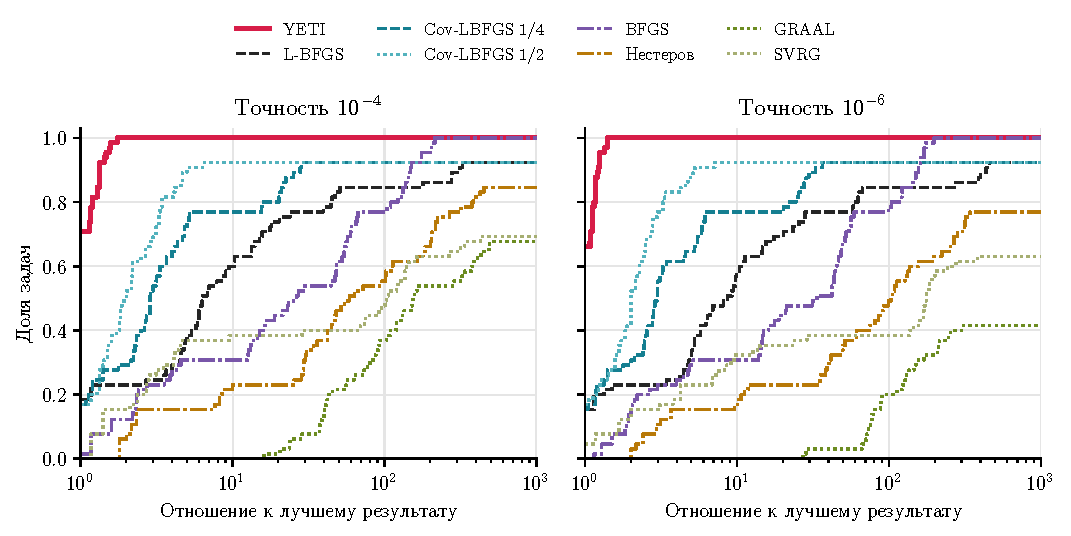
\includegraphics[width=\linewidth]{figures/profiles.pdf}
 \caption{Доля из 65 задач, на которых число запросов не превышает
 лучший результат более чем в $\tau$ раз \citep{dolan2002profiles}. При $\tau=1$ учитываются
 все первые места, включая разделённые; неудачные запуски остаются
 в знаменателе.}
 \label{fig:exp-profiles}
\end{figure}

\begin{table}[!htbp]
 \centering\small
 \setlength{\tabcolsep}{2.3pt}
 \begin{tabular}{@{}lrrrrrrrr@{}}
 \toprule
 Семейство & YETI & L-BFGS & Cov-LBFGS & Cov-LBFGS & BFGS & Нестеров & GRAAL & SVRG\\
 & & (50) & $1/4$ & $1/2$ & & & &\\
 \midrule
 \experimentrows{tables/series65.tex}
 \bottomrule
 \end{tabular}
 \caption{Медиана числа проходов до относительной точности $10^{-6}$
 по пяти экземплярам. «---» означает неудачу хотя бы на одном экземпляре,
 жирным выделен минимум до округления. $\kappa$ --- число обусловленности
 ковариации признаков, $n\times d$ --- число компонент и размерность.}
 \label{tab:exp-series}
\end{table}

Результаты на основном наборе приведены в таблицах~\ref{tab:exp-chains}
и~\ref{tab:exp-glm}. В дополнительных запусках YETI на пяти
синтетических пуассоновских экземплярах медианы числа проходов равны
4, 5 и 5 при $n=2000$, $20000$ и $100000$;
диапазоны --- 4--5, 5--7 и 5--8 соответственно.

\begin{table}[!htbp]
 \centering\small
 \setlength{\tabcolsep}{4pt}
 \begin{tabular}{@{}lrrrrrrrr@{}}
 \toprule
 & \multicolumn{4}{c}{S, длина $T$} & \multicolumn{4}{c}{X, длина $T$}\\
 \cmidrule(lr){2-5}\cmidrule(l){6-9}
 Метод & 8 & 16 & 32 & 64 & 8 & 16 & 32 & 64\\
 \midrule
 \experimentrows{tables/chains.tex}
 \bottomrule
 \end{tabular}
 \caption{Число проходов до относительной точности $10^{-2}$
 на цепочках. Жирным выделен минимум до округления;
 «---» означает, что допуск не достигнут за отведённое число проходов.}
 \label{tab:exp-chains}
\end{table}

\begin{table}[!htbp]
 \centering\small
 \setlength{\tabcolsep}{4pt}
 \begin{tabular}{@{}crrrrrrr@{}}
 \toprule
 & & \multicolumn{3}{c}{До $10^{-2}\widehat\Delta$}
 & \multicolumn{3}{c}{До собственного критерия}\\
 \cmidrule(lr){3-5}\cmidrule(l){6-8}
 Семейство & $T$ & YETI & Без & Случайные & YETI & Без & Случайные\\
 & & & предложений & предложения & & предложений & предложения\\
 \midrule
 \experimentrows{tables/insurance.tex}
 \bottomrule
 \end{tabular}
 \caption{Число проходов при трёх вариантах эвристики.
 Для собственного критерия используется $\varepsilon=10^{-3}\widehat\Delta$.
 «---» означает, что он не выполнен за 200000 проходов.}
 \label{tab:exp-insurance}
\end{table}

\begin{table}[!htbp]
 \centering\small
 \begin{tabular}{@{}lrrrrr@{}}
 \toprule
 & \multicolumn{3}{c}{Синтетические задачи, $n$}
 & Bike & freMTPL2\\
 \cmidrule(lr){2-4}
 Метод & $2000$ & $20000$ & $100000$ & Sharing & freq\\
 \midrule
 \experimentrows{tables/glm.tex}
 \bottomrule
 \end{tabular}
 \caption{Число проходов до относительной точности $10^{-4}$
 на пуассоновских моделях. Обозначения как в табл.~\ref{tab:exp-chains}.}
 \label{tab:exp-glm}
\end{table}
\FloatBarrier

\subsection{Проверка остановки}

На 65 задачах при $\varepsilon=10^{-6}\widehat\Delta$
не менее 90\% запусков завершаются не позднее чем за 37 проходов.
В 63 из 65 запусков YETI останавливается уже в первом эвристическом
блоке. Основной проксимальный шаг понадобился только на двух экземплярах
с редкими признаками при $n=50000$: он выполнен 4 и 8 раз.
На основном наборе все 45 запусков (24 на цепочках и 21 на регрессии)
завершились до первого такого шага.
Рисунок~\ref{fig:exp-certificate} показывает два дополнительных запуска
с более строгим допуском.

\begin{figure}[!htbp]
 \centering
 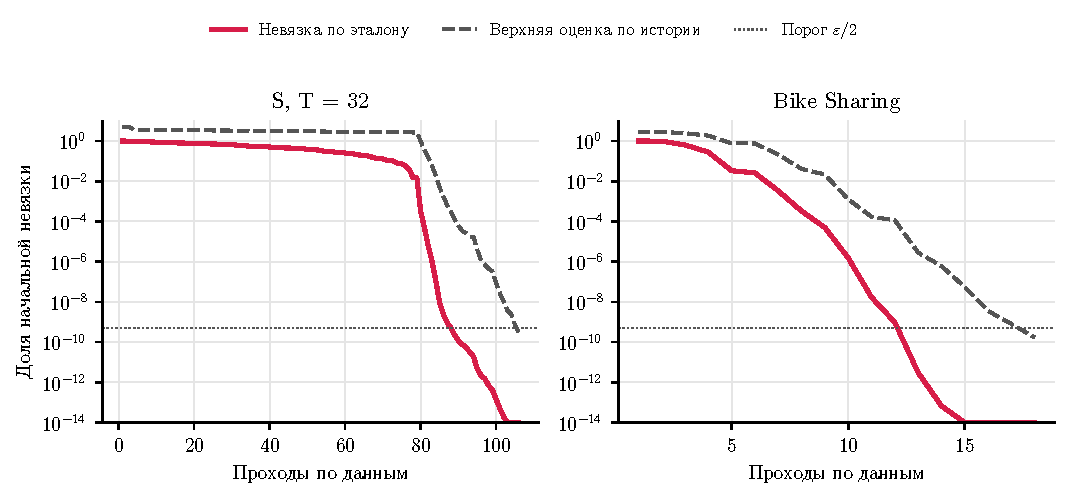
\includegraphics[width=\linewidth]{figures/certificate.pdf}
 \caption{Невязка относительно эталона и её верхняя оценка по истории
 при $\varepsilon=10^{-9}\widehat\Delta$. Все величины делятся на
 $\widehat\Delta$; пунктир --- порог $\varepsilon/2$.
 Значения ниже $10^{-14}$ показаны на нижней границе шкалы.}
 \label{fig:exp-certificate}
\end{figure}

В таблице~\ref{tab:exp-insurance} сопоставлены обычная эвристика,
блок из одного проверочного прохода без предложений и блок, предлагающий
случайные точки допустимого шара. В последнем варианте каждый блок расходует
весь разрешённый лимит: 243--264 прохода.
Общее ограничение составляет 60000 проходов в режиме без предложений
и 200000 --- со случайными предложениями.

Допуск $10^{-2}\widehat\Delta$ достигнут во всех запусках.
Отключение предложений эвристики увеличивает число проходов до допуска
примерно в 41--58 раз, а случайные предложения --- ещё примерно
в 19--54 раза относительно режима без предложений. Таким образом,
в этих опытах основной выигрыш даёт эвристика. Однако её матричные
операции могут быть дорогими, поэтому выигрыш в числе запросов
не обязательно означает такой же выигрыш во времени.
На X при $T=16$ собственный критерий не выполнен за отведённое
число проходов. Ограничение длины блока не устраняет затрат
на бесполезные предложения.
\FloatBarrier
